
\section{General Background}
This section summarizes a general background in \ac{UOWC} systems.

\subsection{Light Propagation in Water}
This section lists with short descriptions the issues \ac{UOWC}
communications face underwater.

\subsubsection{Absorption and Scattering}
A small fraction of light will be absorbed, and another part scattered,
by the water. This becomes more prevalent as the water type degrades,
thus propagation is far more challenging.

\subsubsection{Turbulence}
The refraction index can vary along the propagation path due to
fluctuations in the density, salinity and temperature of the underwater
environment. This is known as scintillation and will degrade performance.

\subsubsection{Pointing and Alignment}
Optical beams are very narrow and thus LOS must be maintained for
reliable link performance. Tracking is required between nodes to
maintain this.

\subsubsection{Background Noise}
As the visible spectrum of light is being used, noise from other light
sources including the Sun can have an effect. In general, deep ocean is
less noisy than harbor side.

\subsubsection{Multipath interference and dispersion}
Multipath interference is produced when an optical signal reaches the
detector after encountering multiple scattering objects or reflections
from other underwater bodies. The signal can be time dispersed thus
decreasing the symbol rate due to \ac{ISI}. It is very dependent on the
operating conditions, and has been concluded that this effect is only
really present in highly turbid environments. Spatial diversity may help
to reduce the effects of multipath interference.

\subsubsection{Physical obstructions}
Anything that might get in the way such as marine animals will cause
momentary loss of signal at the receiver. The light will also attract
marine animals, especially at depth. Error correction, signal processing
techniques and redundancy measures are required to ensure re-transmission
of data when lost.

\subsection{Water Types}
The literature classifies water types in \ac{UOWC} into these main classes.

\subsubsection{Pure Water and Pure Sea Water}
Pure water is the cleanest water type and has no suspended particulate
matter. Pure sea water is pure water but with the addition of salts,
although this is assumed to be negligible in visible spectrum, thus
making pure sea water and pure water equivalent.

\subsubsection{Coastal Ocean}
Coastal ocean displays more severe absorption and scattering due to the
increased concentration of dissolved particles.

\subsubsection{Turbid Harbor}
This is the most hostile environment for optical communications,
with the highest concentration of suspended and dissolved particles
leading to increased absorption and scattering.


\subsection{Configurations of UOWC}
There are 4 types of link configurations with regards to \ac{UOWC}.

\subsubsection{Point to Point \ac{LOS}}
This is the most typical configuration. Both nodes employ the same
transceiver and light sources. Typically the beam angles are narrow, thus
requiring precise pointing between nodes.

\begin{figure}[H]
  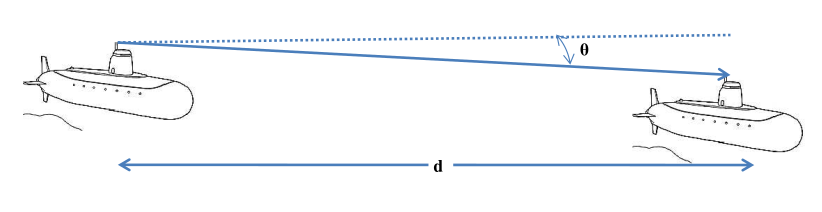
\includegraphics[width=0.8\textwidth]{los-link.png}
  \caption{\ac{LOS} link \cite{kaushal_kaddoum}}
  \label{fig:los-link}
\end{figure}

\subsubsection{Diffused \ac{LOS}}
A point to point link with a large divergence angle allows a signal to be
'broadcast' from one node to multiple remote nodes. Attenuation will be large
though due to the increased interaction area with the water. This is useful
only if short communication distances and lower data rates are required.

\begin{figure}[H]
  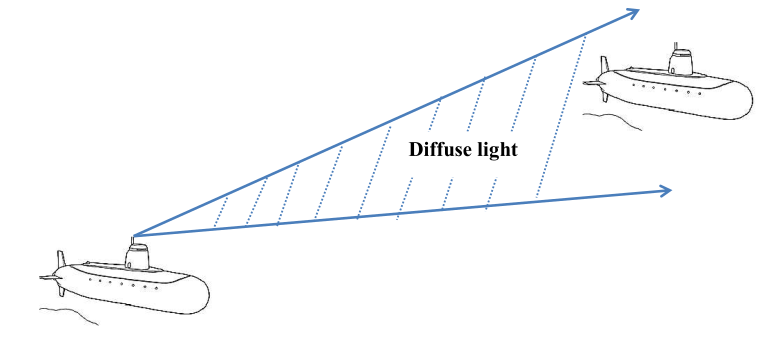
\includegraphics[width=0.8\textwidth]{diffused-link.png}
  \caption{Diffused link \cite{kaushal_kaddoum}}
  \label{fig:diffused-link}
\end{figure}

\subsubsection{Retro-reflector \ac{LOS}}
Instead of having both ends transmit a signal, the remote node reflects back
the received light whilst encoding its response on it. This is ideal for nodes
with low power and weight requirements, but the signal will degrade
significantly due to backscatter and additional attenuation through the water.

\begin{figure}[H]
  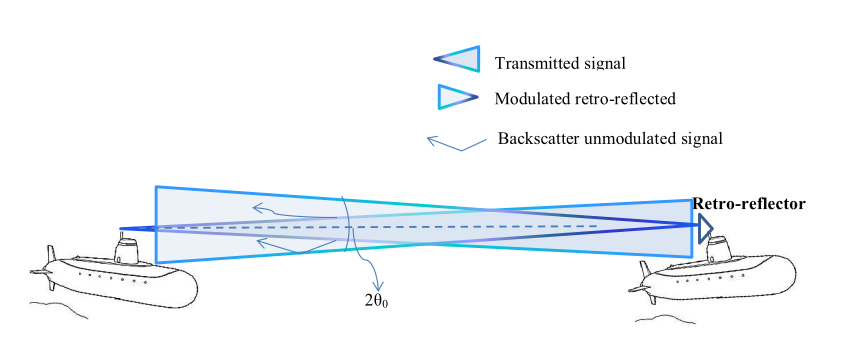
\includegraphics[width=0.8\textwidth]{retro-reflector-link.png}
  \caption{Retro-reflector link \cite{kaushal_kaddoum}}
  \label{fig:retro-reflector-link}
\end{figure}

\subsubsection{\ac{NLOS}}
The signal can be 'bounced' off the sea surface, allowing transmissions to
propagate further if there are underwater obstacles present. Of course, the
light will be reflected in a somewhat random way depending on wind or other
turbulence sources, causing signal dispersion and degradation.

\begin{figure}[H]
  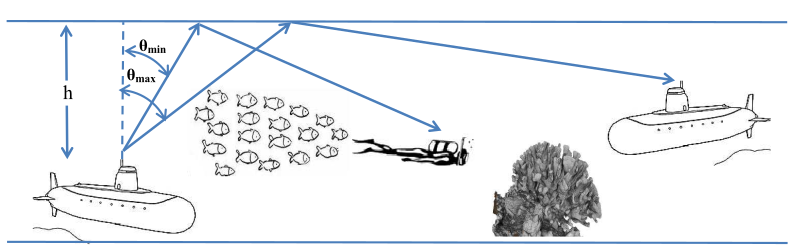
\includegraphics[width=0.8\textwidth]{nlos-link.png}
  \caption{\ac{NLOS} link \cite{kaushal_kaddoum}}
  \label{fig:nlos-link}
\end{figure}

